%%% START A [ 443 words ]

\subsection{Motor Programs}

In this final technical section, we sketch out a possible solution to the problem of motion planning in order to illustrate how an engineer might go about utilizing research in neuroscience to solve a system-wide problem. While we don't directly discuss the problem of automated programming, it is exactly this problem in the context of the programmer's apprentice that motivates our interest in the problem of motion planning.

Our brains derive much of their utility from exploiting distributed representations and parallel processing. Even so, in big brains it is often useful bring representations from distant parts of the brain together and necessary to perform some computations serially with the results from one computation feeding into another. We have evolved machinery that makes it possible for us to do both by making better use of existing memory systems and adapting circuits optimized for movement in order to communicate, plan and perform abstract reasoning.

The mammalian brain makes extensive use of topographically organized representations, often contructing multiple maps with same topographic organization that can be aligned with one another to construct more abstract representations that retain the locality relationships of their constituent maps~\cite{WandelletalNEURON-07,WandelletalPTRS-B-05}. 

The basal ganglia have access to the sensorimotor areas of the cerebral cortex by way of the thalamus and the striatum, the latter being part of the basal ganglia. The thalamus consists of a set of nuclei that map specific subcortical inputs to the cortex and receive feedback from the same cortical areas. The striatum assists in coordinating cognitive functions, including both motor and action planning.

\begin{center}
  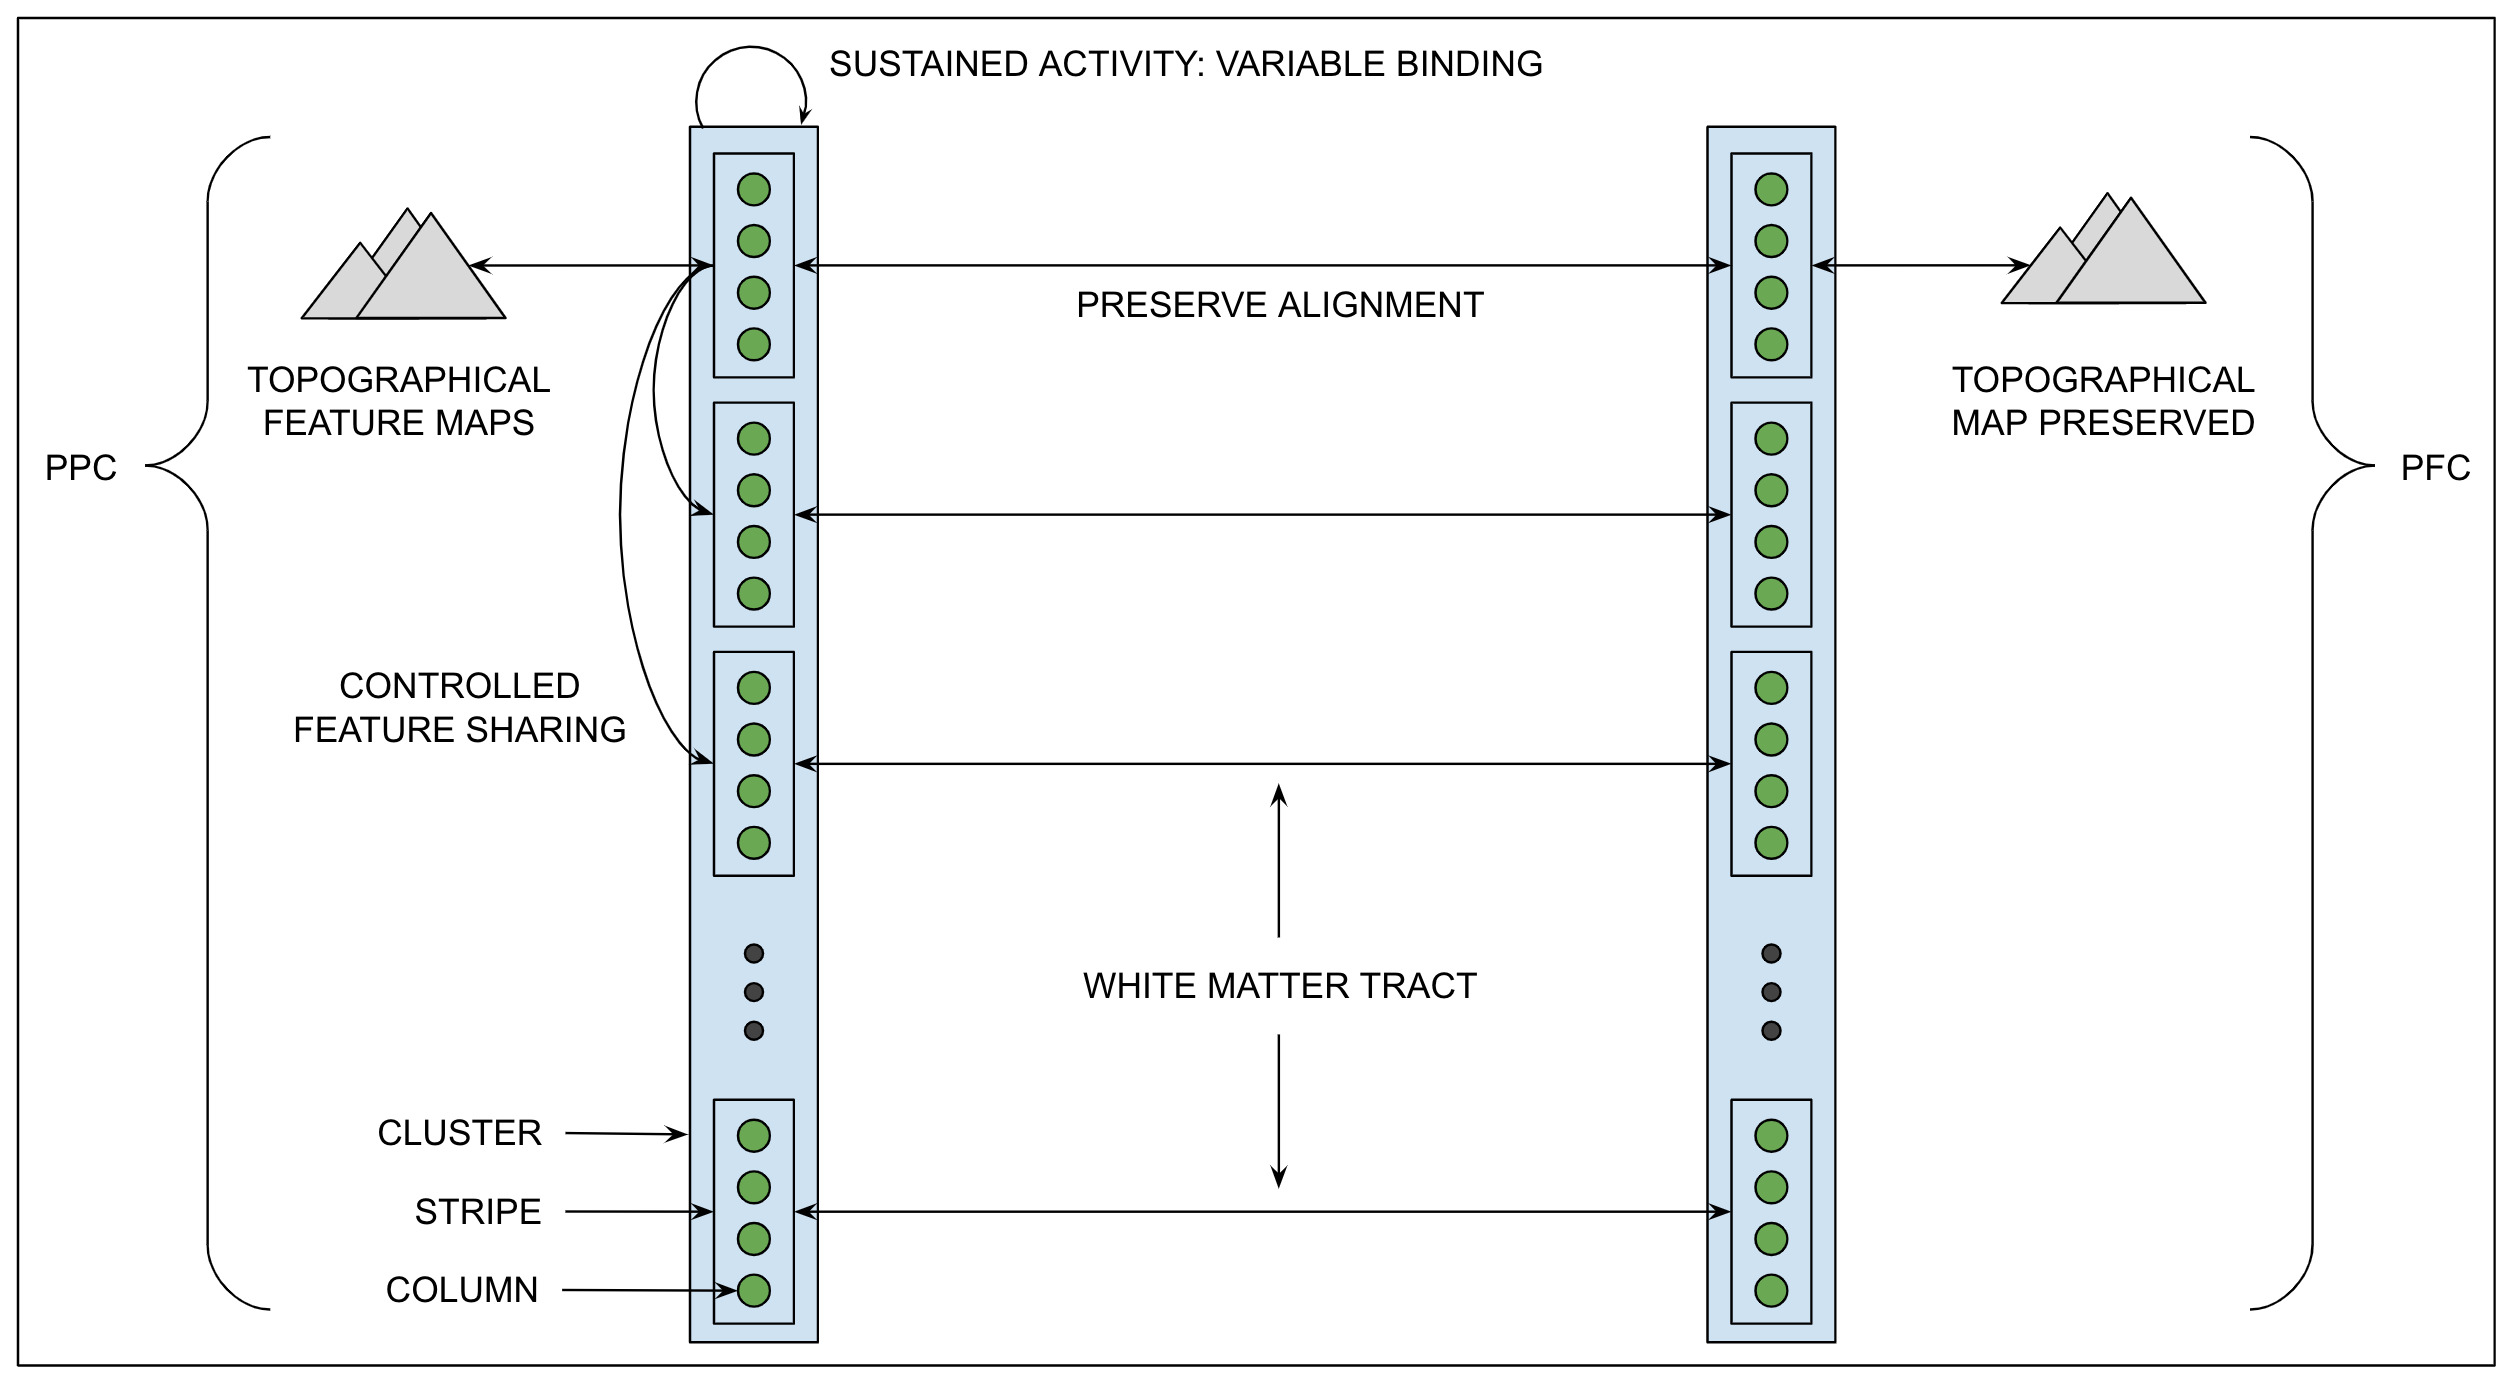
\includegraphics[width=200pt]{./figures/Columns_Stripes_Clusters_Topographic_Maps.jpg}
\end{center}

The striatum's distinctive striated appearance is due to its arrangement of specialized circuits called {\it{stripes}} that enable the basal ganglia to select and transfer information to other locations in the cortex that have similarly functioning circuits, preserving essential topographical features in the process~\cite{BarbasandGarcia-CabezasCOiN-16,LewisetalJNC-02}.

Each stripe is composed of columnar-shaped circuits called {\it{minicolumns}} that encode patterns of coordinated activity originating elsewhere in the cortex so it can brought together in one place for processing. These patterns of activity can be stored indefinitely providing a working memory system that supports a simple yet powerful method for binding variables and composing their values~\cite{OReillyetalCCN-12}.

Stripes are grouped in {\it{clusters}} that map to other clusters often by way of white-matter tracts that connect distant sensory and motor areas. Information is transferred preserving its topographic structure so processed information resulting from motion planning or other cognitive functions can be mapped back to its origin to support learning.

%%% STOP A 
